\section{Unit 1}
\subsection{Lecture 1: Systems of Linear Equations [1.1-1.2]}

A system of linear equations is when you have more than 1 equation with more than 1 unknown.

\begin{example}{}{}
    Solve the following system:
    \[
        \begin{cases}
            x_1 + 2x_2 &= 5 \\
            2x_1 + x_2 &= 4
        \end{cases}
    \]
    \begin{solution}
        \begin{align*}
            x_1 + 2x_2 = 5 &\Rightarrow x_1 = 5-2x_2 \\
            2x_1 + x_2 = 4 &\Rightarrow 2(5-2x_2) + x_2 = 4 \Rightarrow 10-3x_2=4 \\ 
            &\Rightarrow x_2=2 \\
            &\Rightarrow x_1 = 1
        \end{align*}
    \end{solution}
\end{example}

Note that the solution to the previous system $(x_1, x_2) = (1, 2)$ also corresponds to the point of intersection of the lines that each equation represents. This then implies that non-parallel lines have a single solution, paralell lines have no solutions, and scalar multiples of the same line have infinitely many solutions.

\begin{example}{Systems with Different Number of Solutions}{}
    \begin{enumerate}
        \item One Solution:
        \[
            \begin{cases}
                x_1 + 2x_2 &= 5 \\
                2x_1 + x_2 &= 4
            \end{cases} 
        \]

        \item No solution:
        \[
            \begin{cases}
                x_1 + 2x_2 &= 5 \\
                2x_1 + 4x_2 &= 6
            \end{cases}
        \]

        \item Infinite Solutions
        \[
            \begin{cases}
                x_1 + 2x_2 &= 5 \\
                2x_1 + 4x_2 &= 10
            \end{cases}
        \]
    \end{enumerate}
\end{example}

\begin{impbox}{Elementary Row Operations}
    Consider the system 
    \[\begin{cases}
        &E_1 \\
        &E_2 \\
        &\vdots \\
        &E_n
    \end{cases}\]
    Where $E_i$ is the $i$-th equation. Then the following operations on the system \textbf{do not change the solution}
    \begin{enumerate}
        \item Changing the order of equations: $E_i \leftrightarrow E_j$ where $i \ne j$ for the $i$-th and $j$-th equation
        \item Scaling equations: $E_i \rightarrow \lambda E_i$ where $\lambda\in\RR\left(\lambda \ne 0\right)$
        \item Combining equations: $E_i \rightarrow E_i + \lambda E_j$ where $i \ne j$ and $\lambda \in \RR \left(\lambda \ne 0\right)$
    \end{enumerate}
\end{impbox}

\begin{example}{}{}
    Solve the following system:
    \[\begin{cases}
        E_1 &= x_1 + 2x_2 = 5 \\
        E_2 &= 2x_1 + x_2 = 4
    \end{cases}\]
    \begin{solution}
        \begin{align*}
            -2E_1 &= -2x_1 - 4x_2 = -10 \\
            E_2 - 2E_1 &= (2x_1 - x_2) - 2x_1 - 4x_2 = 4-10 \\
            &\Rightarrow -3x_2 = -6 \\
            &\Rightarrow x_2 = 2 \\
            &\Rightarrow x_1 = 1
        \end{align*}
    \end{solution}
\end{example}

\begin{defbox}{Matricies}
    A \textbf{matrix} is a rectangular array of numbers arranged in rows and columns. A matrix $A$ has size $m \times n$ if it has $m$ \textbf{rows} and $n$ \textbf{columns}. A matrix is written as
    \[\underset{m \times n}{A} = \begin{pmatrix}
    a_{11} & a_{12} & \dots & a_{1n} \\
    a_{21} & a_{22} & \dots & a_{2n} \\
    \vdots & & \ddots & \vdots \\
    a_{m1} & a_{m2} & \dots & a_{mn}
    \end{pmatrix}\]
    Where each $a_{ij}$ is called an element of the matrix. $i$ denotes the row and $n$ denotes the column of the element.
\end{defbox}

With this in mind, note that we can represent the previous system as a matrix:
\[\begin{pmatrix}
    1 & 2 & 5 \\
    2 & 1 & 4
\end{pmatrix}\]
where each row represents an equation and each element corresponds to either the coefficent of a variable or the solution. With this system in matrix form we can manipulate the rows as follows:
\[
    \begin{pmatrix}
        1 & 2 & 5 \\
        2 & 1 & 4
    \end{pmatrix} 
    \xrightarrow[R_2 \rightarrow R_2 - 2R_1]{} 
    \begin{pmatrix}
        1 & 2 & 5 \\
        0 & -3 & -6
    \end{pmatrix} 
\]
Since each row corresponds to an equation, if we take a look at the bottom row we can see 
\[ -3x_2 = -6 \Rightarrow x_2 = 2 \Rightarrow x_1 = 1\]
Thus allowing us to reach the same final answer with a lot less hassle. 

\begin{impbox}{General Form of a System of Linear Equations}
    Consider any system of linear equations in the form 
    \[
        \begin{cases}
            a_{11}x_{1} + a_{12}x_{2} + \dots + a_{1n}x_n &= b_1 \\
            a_{21}x_{1} + a_{22}x_{2} + \dots + a_{2n}x_n &= b_2 \\
            \vdots \\
            a_{m1}x_{1} + a_{m2}x_{2} + \dots + a_{mn}x_n &= b_m \\
        \end{cases} 
    \]
    Now, notice we can rewrite this as a matrix:
    \[
        A = \begin{amatrix}{4}
            a_{11} & a_{12} & \dots & a_{1n} & b_1 \\
            a_{21} & a_{22} & \dots & a_{2n} & b_2 \\
            \vdots & & \ddots & \vdots & \vdots \\
            a_{m1} & a_{m2} & \dots & a_{mn} & b_m
        \end{amatrix}
    \]
    Everything to the \textbf{left} of the solid line is refered to as the \textit{coefficent matrix}. $A$ itself is referred to as the \textbf{augmented matrix} for the system.
\end{impbox}

\begin{defbox}{Row Echelon Form}
    Given a matrix $A$, $A_{\text{REF}}$ is an equivalent matrix that satisfies the following properites:
    \begin{enumerate}
        \item All zero rows are below non-zero rows
        \item each next leading element is in the column to the right of the previous leading element (called pivots)
    \end{enumerate}
    Note that the \textbf{leading element} of a row is simply the first non-zero element in that row. 
\end{defbox}

A matrix can also be put in RREF (reduced row echelon form) if it is alreay in REF, each pivot is $1$, and the only non-zero element in the pivot column is the pivot. This would be $A_{\text{RREF}}$. Now, lets try to combine all we've done by applying basic ERO to a simple matrix to put it in REF. 

\begin{example}{Basic REF}{ref}
    Consider the system 
    \[
        \begin{cases}
            x_1 + 2x_2 &= 5 \\
            2x_1 + x_2 = 4
        \end{cases} 
    \]
    Find $\begin{amatrix}{1} A & B \end{amatrix}$
    \begin{solution}
        It's augmented matrix can be put into REF as follows
        \[
            \begin{amatrix}{1}
                A & B
            \end{amatrix}
            = 
            \begin{amatrix}{2}
                1 & 2 & 5 \\
                2 & 1 & 4
            \end{amatrix}
            \xrightarrow[R_2 \rightarrow R_2 - 2R_1]{} 
            \begin{amatrix}{2}
                1 & 2 & 5 \\
                0 & -3 & -6
            \end{amatrix}
            = 
            \begin{amatrix}{1}
                A & B
            \end{amatrix}_{\text{REF}}
        \]
    \end{solution}
\end{example}

\begin{example}{Basic RREF}{}
    Consider again the system from ex~(\ref{th:ref}) and find the RREF of the augmented matrix.
    \begin{solution} 
        Notice we can put it into RREF as follows:
        \[
            \begin{amatrix}{1}
                A & B
            \end{amatrix}_{\text{REF}}
            =  
            \begin{amatrix}{2}
                1 & 2 & 5 \\
                0 & -3 & -6
            \end{amatrix}
            \xrightarrow[R_2 \rightarrow -\frac{1}{3}R_2]{} 
            \begin{amatrix}{2}
                1 & 2 & 5 \\
                0 & 1 & 2
            \end{amatrix}
            \xrightarrow[R_1 \rightarrow R_1 - 2R_2]{} 
            \begin{amatrix}{2}
                1 & 0 & 1 \\
                0 & 1 & 2
            \end{amatrix}
            = 
            \begin{amatrix}{1}
                A & B
            \end{amatrix}_{\text{RREF}}
        \]
    \end{solution}
\end{example}

It's important to note that the RREF for any given matrix is \textit{unique}.

\begin{example}{Solve the System}{}
    Solve the system 
    \[
        \begin{cases}
            x_1 + 2x_2 - x_3 &= 2 \\
            2x_1 + x_2 + x_3 &= 1 \\ 
            x_1 - x_2 + 2x_3 &= -1
        \end{cases}
    \]
    \begin{solution}
        \begin{align*}
            \begin{cases}
                x_1 + 2x_2 - x_3 &= 2 \\
                2x_1 + x_2 + x_3 &= 1 \\ 
                x_1 - x_2 + 2x_3 &= -1
            \end{cases}
            = 
            \begin{amatrix}{3}
                1 & 2 & -1 & 2 \\
                2 & 1 & 1 & 1 \\
                1 & -1 & 2 & -1
            \end{amatrix} &\xrightarrow[\substack{R_2 \to R_2 - 2R_1 \\ R_3 \to R_3 - R_1}]{} 
            \begin{amatrix}{3}
                1 & 2 & -1 & 2 \\
                0 & -3 & 3 & -3 \\
                0 & -3 & 3 & -3
            \end{amatrix} \\
            &\xrightarrow[R_3 \to R_3 - R_2]{}
            \begin{amatrix}{3}
                1 & 2 & -1 & 2 \\
                0 & -3 & 3 & -3 \\
                0 & 0 & 0 & 0
            \end{amatrix} \\
        \end{align*}
        Now because there is no pivot in the third column of our matrix, $x_3$ is what's known as a `free variable'. All this means is that $x_3$ can take on any value, we'll notate this by $x_3 = t$ with $t \in \RR$.
        \begin{align*}
            &\Rightarrow\begin{cases}
                x_3 &= t \\
            -3x_2 + 3x_3 &= -3 \\
            x_1 + 2x_2 - x_3 &= 2
            \end{cases} \\
            &\Rightarrow X_{\text{gen}} = \begin{pmatrix}
                -t \\
                1 + t \\
                t
            \end{pmatrix}
        \end{align*}
    \end{solution}
\end{example}

\subsection{Lecture 2: Vector and Matrix Equations [1.3-1.4]}

As a reminder from last time, given a system with an augmented matrix 
$\begin{amatrix}{1}
    A & B
\end{amatrix}$
the system will have
\begin{enumerate}
    \item \underline{no} solutions if there is a pivot in the last column of 
    $\begin{amatrix}{1}
        A & B
    \end{amatrix}_{\text{REF}}$
    \item \underline{one} solution if $\begin{amatrix}{1}
        A & B
    \end{amatrix}_{\text{REF}}$ is $m \times n$ with $n$ pivots (and no pivots in the last column)
    \item \underline{infinite} solutions if $\begin{amatrix}{1}
        A & B
    \end{amatrix}_{\text{REF}}$ is $m \times n$ with less than $n$ pivots (and no pivots in the last column)
\end{enumerate}

\begin{defbox}{Vectors}{}
    For a vector $\vec{AB}$, point $A$ is the tail and point $B$ is the head. Two vectors, $\vec{AB}$ and $\vec{CD}$ are equal if, and only if, their magnitude and directions are equal. Vectors in $\RR^{2}$ can be notated as $\big(\begin{smallmatrix} a_1 \\ a_ 2\end{smallmatrix}\big)$ where the point $(a_1, a_2)$ is the head and the tail is (usually) assumed to the origin. Generally, for $\RR^{n}$ we have $\begin{pmatrix} x_1 \\ \vdots \\ x_n \end{pmatrix}$ which will always have size $n \times 1$.
\end{defbox}

Since we can represent vectors as matricies, we can perform the standard matrix operations on them:

\begin{impbox}{Matrix Operations}{}
    Let $A$ and $B$ be matricies. Then
    \begin{enumerate}
        \item $A + B = C$ where $A$ and $B$ are the same size. This addition is defined as $c_{ij} = a_{ij} + b_{ij}$
        \item $\lambda A = \hat{A}$ where $\hat{a_{ij}} = \lambda a_{ij}$ for $\lambda \in \RR$
        \item $A + (-A) = \hat{0}$ where $\hat{0}$ is the \underline{zero-matrix} which has the same size as $A$ with each element being $0$
        \item Consider matricies $\underset{m \times n}{A}$ and $\underset{n\times 1}{X}$, then $AX$ is defined as
        \[
            \underset{m \times 1}{A} = 
            \begin{pmatrix}
                a_{11}x_{1} & a_{12}x_2 & \dots & a_{1n}x_n \\
                a_{21}x_1 & a_{22}x_2 & \dots & a_{2n}x_n \\
                \vdots & & \ddots & \vdots \\
                a_{m1}x_1 & a_{m2}x_2 & \dots & a_{mn}x_n
            \end{pmatrix}
            \text{ if }
            \underset{m\times n}{A} = 
            \begin{pmatrix}
                a_{11} & a_{12} & \dots & a_{1n} \\
                a_{21} & a_{22} & \dots & a_{2n} \\
                \vdots & & \ddots & \vdots \\
                a_{m1} & a_{m2} & \dots & a_{mn}
            \end{pmatrix}
            \text{ and }
            \underset{n \times 1}{X} = 
            \begin{pmatrix}
                x_1 \\
                x_2 \\
                \vdots 
                \\ 
                x_n
            \end{pmatrix}
        \]
    \end{enumerate}
\end{impbox}

\begin{example}{Basic Matrix Multiplication}{}
    Consider the the matricies 
    \[ 
        \underset{2 \times 3}{A} = 
        \begin{pmatrix}
            1 & -1 & 2 \\
            3 & 4 & 5 
        \end{pmatrix} 
        \text{ and }
        \underset{3 \times 1}{B} = 
        \begin{pmatrix}
            2 \\
            4 \\
            7
        \end{pmatrix}
    \]
    Find $AB$.
    \begin{solution}
        \[ 
            \underset{2 \times 1}{AB} = 
            \begin{pmatrix}
                (1 * 2) + (-1 * 4) + (2 * 7) \\
                (3 * 2) + (4 * 4) + (5 * 7) 
            \end{pmatrix}
            = 
            \begin{pmatrix}
                12 \\
                57
            \end{pmatrix}
        \]
    \end{solution}
\end{example}

It's important to note that an alternative form of defining matrix multiplication is as follows:
\[
    AX = 
    x_1\begin{pmatrix}
        a_{11} \\ a_{21} \\ \vdots \\ a_{m1}
    \end{pmatrix}
    + x_2\begin{pmatrix}
        a_{12} \\ a_{22} \\ \vdots \\ a_{m2}
    \end{pmatrix}
    + \dots + 
    x_n\begin{pmatrix}
        a_{m1} \\ a_{m2} \\ \vdots \\ a_{mn}
    \end{pmatrix}
\]
This is known as the \textbf{linear combination of vectors}.

\begin{defbox}{Linear Combination of Vectors}{}
    Let $\braces{\vec{u_1}, \vec{u_2}, \dots, \vec{u_k}}$ be a set of vectors from $\RR^{n}$. Then, 
    \[
        c_1\vec{u_1} + c_2\vec{u_2} + \dots + c_k\vec{u_k}, \hspace{0.2in} (c_1, c_2, \dots, c_k \in \RR) 
    \]
    is called the \textbf{linear combination of vectors} $\vec{u_1}, \vec{u_2}, \dots, \vec{u_k}$.
\end{defbox}

We can combine the previous two definitions of matrix multiplication and the linear combination of vectors to get this next fact: if we consider a vector 
\[(\vec{u_k}) = \begin{pmatrix} u_{1k} \\ u_{2k} \\ \vdots \\ u_{nk} \end{pmatrix}\]
then, $c_1\vec{u_1} + c_2\vec{u_2} + \dots + c_k\vec{u_k} = AX$ where
\[
    A = 
    \begin{pmatrix}
        \left(\vec{u_1}\right) & \left(\vec{u_2}\right) & \dots & \left(\vec{u_k}\right)
    \end{pmatrix}
    \text{ and }
    X = \begin{pmatrix}
        c_1 \\ c_2 \\ \vdots \\ c_k
    \end{pmatrix}
\]

This is especially important when working with systems of equations as we can represent systems as linear combinations of vectors. Given any general system we can rewrite it as a linear combination of vectors as such
\[ 
    \left.\begin{cases}
        a_{11}x_1 + a_{12}x_2 + \dots + a_{1n}x_n &= b_1 \\
        a_{21}x_1 + a_{22}x_2 + \dots + a_{2n}x_n &= b_1 \\
        \vdots & \\
        a_{m1}x_1 + a_{m2}x_2 + \dots + a_{mn}x_n &= b_1 \\
    \end{cases}\right] \Leftrightarrow AX = B
\]
$B$ is said to be a \textit{linear combination of columns of $A$} if, and only if, $A$ and $B$ are \textbf{compatible}. For $A$ and $B$ to be compatible essentially just means that $\begin{amatrix}{1} A & B\end{amatrix}_{\text{REF}}$ has no pivots in the last column.

\begin{defbox}{Span}{}
    $c_1\vec{v_1} + c_2\vec{v_2} + \dots + c_k\vec{v_k} = \text{Span}\braces{\vec{v_1}, \vec{v_2}, \dots, \vec{v_k}}$ where $c_1, c_2, \dots, c_k$ are \underline{all} possible numbers
\end{defbox}

For a single vector $\vec{v}$, $\text{Span}\braces{\vec{v}}$ is simply the set containing all scaled multiples of $\vec{v}$.

\begin{example}{Span of Two Vectors}{}
    Notice that $\text{Span}\braces{\begin{pmatrix} 1 \\ 2\end{pmatrix}, \begin{pmatrix} 3 \\ 4\end{pmatrix}} = \RR^{2}$. This implies that any vector from $\RR^{2}$ can be written as 
    \[ c_1\begin{pmatrix} 1 \\ 2 \end{pmatrix} + c_2\begin{pmatrix} 3 \\ 4\end{pmatrix}\]
    We can prove this fact by considering the augmented matrix for $AX=B$:
    \[ 
        \begin{amatrix}{2}
           1 & 3 & b_1 \\
           2 & 4 & b_2  
        \end{amatrix}
        \xrightarrow[R_2 \to R_2 - 2R_1]{} 
        \begin{amatrix}{2}
            1 & 3 & b_1 \\
            0 & -2 & b_2 - 2b_1
        \end{amatrix}
    \]
    Therefore, since there is no pivote in the last column, this system has a single solution for any vector $B = \begin{pmatrix} b_1 \\ b_2 \end{pmatrix}$
\end{example}

\begin{example}{}{}
    Given the following vectors $\vec{a_1}, \vec{a_2}, \vec{a_3}$ and $\vec{b}$, determine if $\vec{b}$ is a linear combination of $\vec{a_1}, \vec{a_2}, \vec{a_3}$.
    \[
        \vec{a_1} = \begin{pmatrix} 1 \\ -2 \\ 0 \end{pmatrix} 
        \hspace{0.2cm}
        \vec{a_2} = \begin{pmatrix} 0 \\ 1 \\ 2 \end{pmatrix} 
        \hspace{0.2cm}
        \vec{a_3} = \begin{pmatrix} 5 \\ -6 \\ 8 \end{pmatrix} 
        \hspace{0.2cm}
        \vec{b} = \begin{pmatrix} 2 \\ -1 \\ 6 \end{pmatrix} 
        \hspace{0.2cm}
    \]
    We can start by noticing that $\vec{b} = c_1\vec{a_1} + c_2\vec{a_2} + c_3\vec{a_3} \Leftrightarrow A\begin{pmatrix} c_1 \\ c_2 \\ c_3 \end{pmatrix} = \begin{pmatrix} b_1 \\ b_2 \\ b_3 \end{pmatrix}$ where \\ $A = \begin{pmatrix} \left(\vec{a_1}\right) & \left(\vec{a_2}\right) & \left(\vec{a_3}\right) \end{pmatrix}$. Thus, 
    \[ 
        \begin{amatrix}{3}
            1 & 0 & 5 & 2 \\
            -2 & 1 & -6 & -1 \\
            0 & 2 & 8 & 6 
        \end{amatrix} 
        \xrightarrow[R_2 \to R_2 + 2R_1]{}
        \begin{amatrix}{3}
            1 & 0 & 5 & 2 \\
            0 & 1 & 4 & 3 \\
            0 & 2 & 8 & 6 
        \end{amatrix} 
        \xrightarrow[R_3 \to R_3 - 2R_2]{}
        \begin{amatrix}{3}
            1 & 0 & 5 & 2 \\
            0 & 1 & 4 & 3 \\
            0 & 0 & 0 & 0 
        \end{amatrix} 
    \]
    Therefore, since there is no pivot in the final column, $B$ is a linear combination of $A$.
\end{example}

\subsection{Lecture 3: Homogenous Systems of Linear Equations [1.5]}\label{lecture:3}

\begin{defbox}{Homogenous Systems of Linear Equations}{}
    A \textbf{homogenous system of linear equations} is any system in the form 
    \[Ax = \hat{0}\]
    Thus, any system in the form \[Ax = B\] is called a \textbf{non-homogenous system}. 
\end{defbox}

For a non-homogenous system we can follow the steps
\[ Ax = B \Rightarrow \begin{amatrix}{1} A & B \end{amatrix} \xrightarrow[\text{ERO}]{} \begin{amatrix}{1} A & B \end{amatrix}_{\text{REF}} \Rightarrow \text{backwards substitution into the equations}\]
For each non-homogenous system:
\begin{enumerate}
    \item if the augmented matrix has a pivote in the last column, it has no solutions
    \item if $A$ is $m \times n$ and the augmented matrix has less than $n$ pivots, then $Ax=B$ has an infinite amount of solutions
    \item if $A$ is $m \times n$ and the augmented matrix has exactly $n$ pivots then $Ax=B$ has \underline{one} solution
\end{enumerate}
For a homogenous system we can follow similar steps:
\[Ax = \hat{0} \Rightarrow \begin{amatrix}{1} A & 0 \end{amatrix}\xrightarrow[\text{ERO}]{} A_{\text{REF}} \Rightarrow \text{backwards substitution to the equations}\]
Note that since the solution matrix is simply just the zero matrix, we dont need to consider it in our augmented matrix - thats why you see $A_\text{REF}$. Unlike non-homogenous systems there are only two options for solutions:
\begin{enumerate}
    \item $x=\hat{0}$ is \underline{always} a solution, this is called the \textit{trivial solution}. If $A_\text{REF}$ is $m \times n$ large and has $n$ pivots, then $x=\hat{0}$ is the \textbf{only} solution
    \item if $A_{\text{REF}}$ is $m \times n$ and has less than $n$ pivots, then $Ax=\hat{0}$ has an \textbf{infinite} amount of solutions
\end{enumerate}

\begin{example}{Solve the following System}{}
    Solve the below system
    \[\begin{cases}
        x_1 + 2x_2 - 3x_3 + x_4 &= 0 \\
        2x_2 - x_2 + x_3 - 2x_4 &= 0 \\
        3x_1 + x_2 - x_3 + x_4 &= 0
    \end{cases}\]
    We can start by putting this in the form $Ax=\hat{0}$ where 
    \[\underset{3 \times 4}{A} = \begin{pmatrix}
        1 & 2 & -3 & -1 \\
        2 & -1 & 1 & -2 \\
        3 & 1 & -1 & 1
    \end{pmatrix}, \hspace{0.2cm}
    \underset{4 \times 1}{X} = \begin{pmatrix}
        x_1 \\ x_2 \\ x_3 \\ x_4
    \end{pmatrix}\]
    Next, we need to put $A$ into REF: 
    \[
        \underset{3 \times 4}A \xrightarrow[\substack{R_2 \to R_2 - 2R_1 \\ R_3 \to R_3 - 3R_1}]{} 
        \begin{pmatrix}
            1 & 2 & -3 & -1 \\
            0 & -5 & 7 & -4 \\
            0 & -5 & 8 & -2
        \end{pmatrix} 
        \xrightarrow[R_3 \to R_3 - R_2]{}
        \begin{pmatrix}
            1 & 2 & -3 & -1 \\
            0 & -5 & 7 & -4 \\
            0 & 0 & 1 & 2
        \end{pmatrix} 
        = A_{\text{REF}}
    \]
    Since there is no pivot in the fourth column, $x_4$ must be a free variable. We can rename it as $x_4=t$ for $t \in \RR$. Thus
    \[
        \left.\begin{cases}
            x_3 + 2x_4 &= 0 \Rightarrow x_3 = -2t \\
            -5x_2 + 7x_3 - 4x_3 &= 0 \Rightarrow x_2 = -\frac{18}{5}t \\
            x_1 + 2x_2 - 3x_3 + x_4 &0 = 0 \Rightarrow x_1 = \frac{1}{5}t 
        \end{cases}\right]
        \Rightarrow
        X = \begin{pmatrix} \frac{1}{5}t \\ -\frac{18}{5}t \\ -2t \\ t \end{pmatrix}
        \Leftrightarrow 
        \begin{pmatrix}
            1 \\ -18 \\ -10 \\ 5
        \end{pmatrix}t
    \]
    Notice that since $t$ is any arbitary value we can make $t = 5t$ in order to eliminate the fractions. As well, the second matrix with $t$ on the outside is known as the \textit{parametric form} of the solution.
\end{example}

\begin{thm}{}{}
    The general solution of a consisten non-homogenous system $Ax=B$ has the form $X_{\text{gen}} = X_{\text{genhom}} + X_{\text{p}}$ where $X_{\text{genhom}}$ is the general solution of the corresponding homogenous system $Ax=\hat{0}$ and $X_p$ is any particular solution of $Ax=B$.
    \begin{proof}
       Let $X_1$ and $X_2$ be any two solutions of $Ax=B$. That is, 
       \[\left.\begin{cases}
            AX_1 &= B \\
            AX_2 &= B
       \end{cases}\right]
       \Rightarrow AX_1 - AX_2 = 0 \Leftrightarrow A(X_1-X_2) = 0\] 
       Therefore, $X_1 - X_2$ is a solution of the homogenous system. With some clever `renaming' we can see:
       \[X_1 - X_2 = X_{\text{hom}} \Rightarrow X_1 = X_{\text{hom}} + X_2 \Rightarrow X_{\text{gen}} = X_{\text{genhom}} + X_{p}\]
    \end{proof}
\end{thm}

\begin{example}{Solve the System}{}
    \[\begin{cases}
        x_1 + 2x_2 - x_3 &= 4 \\
        2x_1 + x_2 - 2x_3 &= 2 \\
        x_1 + x_2 - x_3 &= 2
    \end{cases}\]
    As always, we start by forming the augmented matrix and putting it into REF:
    \[\begin{amatrix}{3}
        1 & 2 & -1 & -4 \\
        2 & 1 & -2 & 2 \\
        1 & 1 & -1 & 2
    \end{amatrix}
    \xrightarrow[\substack{R_2 \to R_2 - 2R_1 \\ R_3 \to R_3 - R_2}]{}
    \begin{amatrix}{3}
        1 & 2 & -1 & 4 \\
        0 & -3 & 0 & -6 \\
        0 & -1 & 0 & -2
    \end{amatrix}
    \xrightarrow[\substack{R_2 \to -\frac{1}{3}R_2 \\ R_3 \to R_3 - \frac{1}{3}R_2}]{} 
    \begin{amatrix}{3}
        1 & 2 & -1 & 4 \\
        0 & 1 & 0 & 2 \\
        0 & 0 & 0 & 0
    \end{amatrix}
    \] 
    \[
    \xrightarrow[R_1 \to R_1 - 2R_2]{}
    \begin{amatrix}{3}
        1 & 0 & -1 & 0 \\
        0 & 1 & 0 & 2 \\
        0 & 0 & 0 & 0
    \end{amatrix}
    \]
    Now, since there is no pivot in the third column, $x_3$ must be a free variable, so we have $x_3=t$ for $t \in \RR$. Using some very basic backwards substitution we can see that $x_2 = 2$ and $x_1 = x_3 = t$. As well, notice that the final form of the augmented matrix is actually in RREF and not REF, because of how easy it was to put the matrix in RREF from REF, there was almost no reason \textbf{not} to put it into RREF. We can now write our solution vector,
    \[X_{\text{gen}} = \begin{pmatrix} t \\ 2 \\ t\end{pmatrix} = \underbrace{\begin{pmatrix}
    0 \\ 2 \\ 0
    \end{pmatrix}}_{X_p} + t\underbrace{\begin{pmatrix}
    1 \\ 0 \\ 1
    \end{pmatrix}}_{X_{\text{genhom}}}\]
\end{example}

\begin{example}{Find the General Homogenous Solution}{}
    Just to prove the point, lets find the general homogenous solution for the above system, $Ax = \hat{0}$. 
    \[A = \begin{pmatrix}
        1 & 2 & -1 \\
        2 & 1 & -2 \\
        1 & 1 & -1
    \end{pmatrix}
    \xrightarrow[\substack{R_2 \to R_2 - 2R_2 \\ R_3 \to R_3 - R_1}]{} 
    \begin{pmatrix}
        1 & 0 & -1 \\
        0 & 1 & 0 \\
        0 & 0 & 0
    \end{pmatrix} = A_{\text{RREF}} 
    \]
    With backwards substitution we can easily see that $x_3=t$ for $t \in \RR$, $x_2=0$, and $x_1 = t$. So, 
    \[X_{\text{genhom}} = \begin{pmatrix}
        t \\ 0 \\ t
    \end{pmatrix} = t\begin{pmatrix}
        1 \\ 0 \\ 1
    \end{pmatrix}\]
    Which, as expected, is exactly the same vector we saw in the previous example.
\end{example}

\begin{example}{Solve the System}{}
    \[\begin{cases}
        x_1 - 2x_2 + x_3 + x_4 &= 0 \\
        2x_1 + x_2 - 2x_3 + x_4 &= 0 \\
        3x_1 - x_2 - x_3 &= 0 
    \end{cases}\]
    Once again, we must put $A$ into REF:
    \[A \xrightarrow[\substack{R_2 \to R_2 - 2R_1 \\ R_3 \to R_3 - 3R_1}]{} \begin{pmatrix}
        1 & -2 & 1 & -1 \\
        0 & 5 & -4 & 3 \\
        0 & 5 & -4 & 3
    \end{pmatrix}
    \xrightarrow[R_3 \to R_3 - R_2]{} 
    \begin{pmatrix}
        1 & -2 & 1 & 1 \\
        0 & 5 & -4 & 3 \\
        0 & 0 & 0 & 0 
    \end{pmatrix}
    \]
    Now, because there are no pivots in the third and fourth column, $x_3$ and $x_4$ are free variables which makes $x_1$ and $x_2$ our basic variables $\therefore x_3 = t, x_4 = s$ for $s, t \in \RR$
    \[
        \begin{cases}
            5x_2 - 4x_3 + 3x_4 &= 0 \Rightarrow x_2 = \frac{4}{5}x_3 - \frac{3}{5}x_4 = \frac{4}{5}t - \frac{3}{5}s \\
            x_1 - 2x_2 + x_3 - x_4 &= 0 \Rightarrow x_1 = 2x_2 - x_3 + x_4 = 2(\frac{4}{5}t - \frac{3}{5}s) - t + s
        \end{cases} 
    \]
    Before continuing, it's smart to make $t = 5t$ and $s=5s$ in order to eliminate the fractions. Then we have:
    \[X_{\text{gen}} = \begin{pmatrix}
        3t - s \\ 4t - 3s \\ 5t \\ 5s
    \end{pmatrix} = t\begin{pmatrix}
        3 \\ 4 \\ 5 \\ 0 
    \end{pmatrix} + s\begin{pmatrix}
        -1 \\ -3 \\ 0 \\ 0 
    \end{pmatrix}\]
\end{example}

\subsection{Lecture 4: Span of a Set of Vectors [1.3]}
\begin{defbox}{Rank of a Matrix}{}
    Let $\underset{m \times n}{A}$ be a matrix. Then $\text{rank}(A)$ is the number of pivots in $A_{\text{REF}}$. $\text{rank}(A)$ is equivalent to the number of non-zero rows in $A_{\text{REF}}$. 
\end{defbox}

It follows from the definition of $\text{rank}(A)$ that the number of free variables in a system is $n - \text{rank}(A)$. This quanitity is known as $\text{null}(A)$.

If $\underset{n \times n}{A}$ is a matrix such that $\text{rank}(A) = n$, then $A_{\text{REF}} = I$ where $I$ is the identity matrix.

\begin{defbox}{Identity Matrix}{}
    The identity matrix, $I$, is a square matrix which is automatically in RREF and its only non-zero elements are the pivots. For example
    \[I_2 = \begin{pmatrix}
        1 & 0 \\
        0 & 1
    \end{pmatrix}
    \hspace{0.2cm}
    \text{and}
    \hspace{0.2cm}
    I_3 = \begin{pmatrix}
        1 & 0 & 0 \\
        0 & 1 & 0 \\
        0 & 0 & 1
    \end{pmatrix}\]
\end{defbox}

Another important fact about the rank of matrix is that it can only be as great as the minimimum of $n$ and $m$ for a matrix of size $m \times n$. Formally, 
\[ \text{rank}\left(\underset{m \times n}{A}\right) \leq \min\braces{m, n}\]
where $\min\braces{x_1, x_2, \dots, x_n}$ returns the smallest value out of $x_1, x_2, \dots, x_n$.

\begin{defbox}{Span of Vectors from $\RR^{n}$}{}
    The span of a set of vectors from $\RR^{n}$, $\text{Span}\braces{\vec{u_1}, \vec{u_2}, \dots, \vec{u_k}}$ is the set of all possible linear combinations of $\vec{u_1}, \vec{u_2}, \dots, \vec{u_k}$:
    \[AC = c_1\vec{u_1} + c_2\vec{u_2} + \dots + c_k\vec{u_k}, \hspace{0.4cm}\left(c_1, c_2, \dots, c_k \in \RR \right)\]
    where 
    \[
        A = \begin{pmatrix}
            \left(\vec{u_1}\right) & \left(\vec{u_2}\right) & \dots & \left(\vec{u_k}\right) 
        \end{pmatrix}
        \text{ and } 
        C = \begin{pmatrix}
            c_1 \\ c_2 \\ \vdots \\ c_k 
        \end{pmatrix}
    \]
\end{defbox}

The span of the zero vector, is also the zero vector: $\text{Span}\braces{\vec{0}} = \vec{0}$

\begin{example}{Span of a Single Vector}{}
    Consider a vector $u_1 = \begin{pmatrix} 1 \\ 2 \end{pmatrix}$. Then $\Span{\vec{u_1}} = c\vec{u_1}$ for any $c \in \RR$. Geometrically, this is the set of vectors in the same, or opposite, direction as $\vec{u_1}$ with a scaled magnitude. When put together, $\Span{\vec{u_1}}$ gives a line in $\RR^{2}$.
\end{example}

\begin{example}{Span of Two Vectors}{}
    Consider $\vec{u_1} = \begin{pmatrix} 1 \\ 2 \end{pmatrix}$ and $\vec{u_2} = \begin{pmatrix} 1 \\ 1 \end{pmatrix}$. Then, $\Span{\vec{u_1}, \vec{u_2}} = \RR^{2}$ because any vector from $\RR^2$ can be writtin in the form 
    \[
        c_1\vec{u_1} + c_2\vec{u_2} = c_1\begin{pmatrix} 1 \\ 2 \end{pmatrix} + c_2\begin{pmatrix} 1 \\ 2 \end{pmatrix}
    \]
    \begin{proof}
        Consider the system 
        \[
            c_1\begin{pmatrix} 1 \\ 2 \end{pmatrix} + c_2\begin{pmatrix} 1 \\ 2 \end{pmatrix} = \begin{pmatrix} b_1 \\ b_2 \end{pmatrix} 
            \Leftrightarrow 
            \begin{pmatrix}
                1 & 1 \\
                2 & 1
            \end{pmatrix}
            \begin{pmatrix}
                c_1 \\ c_2
            \end{pmatrix}
            = 
            \begin{pmatrix}
                b_1 \\ b_2
            \end{pmatrix}
            \Leftrightarrow 
            A \begin{pmatrix}
                c_1 \\ c_2 
            \end{pmatrix}
            = 
            \begin{pmatrix}
                b_1 \\ b_2
            \end{pmatrix}, 
            \hspace{0.2cm}
            \underset{2 \times 2}{A} = \begin{pmatrix}
                1 & 1 \\
                2 & 1
            \end{pmatrix}
        \]
        Then, the augmented matrix is 
        \[
            \begin{amatrix}{2}
                1 & 1 & b_1 \\
                2 & 1 & b_2
            \end{amatrix}
            \xrightarrow[R_2 \to R_2 - 2R_1]{} 
            \begin{amatrix}{2}
                1 & 1 & b_1 \\
                0 & -1 & b_2 - 2b_1
            \end{amatrix}
            = 
            \begin{amatrix}{1}
                A & B
            \end{amatrix}_{\text{REF}}
        \]
        $\therefore$ since the augmented matrix in REF has no pivots in the final column, the system is compatible and contains a solution for all vectors $\begin{pmatrix} b_1 \\ b_2\end{pmatrix} \in \RR$.
    \end{proof}
\end{example}

Note as well, that we could've written the final justification using the rank of augmented matrix as reasoning: `$\therefore \text{rank}(A) = 2$, so the system is compatible\dots'. As well, note that since $A$ is a square matrix and $\text{rank}(A) = 2$, that also implies that $A_{\text{RREF}} = I_2$ (it should be pretty easy to put $A$ into RREF and see this for yourself).

\begin{example}{Span of Three Vectors}{}
    Consider three vectors
    \[
        \vec{u_1} = \begin{pmatrix}
            1 \\ 2
        \end{pmatrix},
        \hspace{0.2cm}
        \vec{u_2} = \begin{pmatrix}
            2 \\ 4
        \end{pmatrix}, 
        \hspace{0.2cm}
        \vec{u_3} = \begin{pmatrix}
            3 \\ 6
        \end{pmatrix}
    \]
    and consider the span of $\vec{u_1}, \vec{u_2}$ and $\vec{u_3}$, $\Span{\vec{u_1}, \vec{u_2}, \vec{u_3}}$. Now notice that $u_2 = 2u_1$ and $u_3 = 3u_3$. This implies that $\Span{\vec{u_1}, \vec{u_2}, \vec{u_3}} = \Span{\vec{u_1}}$. $u_2$ and $u_3$ are considered `redudant' in the span.
    \begin{proof}
        Consider the matrix representing the vectors of the generation set:
        \[
            \begin{pmatrix}
                1 & 2 & 3 \\
                2 & 4 & 6
            \end{pmatrix}
            \xrightarrow[R_2 \to R_2 - 2R_1]{}
            \begin{pmatrix}
                1 & 2 & 3 \\
                0 & 0 & 0
            \end{pmatrix}
        \]
        $\therefore$ no pivots in the second and third columns implies that the second and third vectors are redudant. 
    \end{proof}
\end{example}


\begin{example}{Span of Three Vectors (again)}
    Now consider $\vec{u_1}, \vec{u_2}, \vec{u_3}$ such that 
    \[
        \vec{u_1} = \begin{pmatrix}
            1 \\ 3
        \end{pmatrix}, 
        \hspace{0.2cm}
        \vec{u_2} = \begin{pmatrix}
            2 \\ 1
        \end{pmatrix}, 
        \hspace{0.2cm}
        \vec{u_3} = \begin{pmatrix}
            4 \\ 6
        \end{pmatrix}
    \]
    Notice that $\Span{\vec{u_1}, \vec{u_2}, \vec{u_3}}$ \textbf{must} be reducible since the corresponding matrix has dimensions $2 \times 3 \Rightarrow \text{rank}{A} \leq \min{2, 3} = 2 \therefore$ (at least) one vector is redudant. We can figure out which one as follows 
    \[
        \underset{2 \times 3}{A} = \begin{pmatrix}
            1 & 2 & 4 \\
            3 & 1 & 6 
        \end{pmatrix}
        \xrightarrow[R_2 \to R_2 - 3R_1]{}
        \begin{pmatrix}
            1 & 2 & 4 \\
            0 & -5 & -6
        \end{pmatrix}
    \]
    Thus, no pivot in the third column implies that the third vector is redudant:
    \[\therefore \Span{\vec{u_1}, \vec{u_2}, \vec{u_3}} = \Span{\vec{u_1}, \vec{u_2}}\]
\end{example}

\begin{example}{Proving a Vector is in a Span}{}
    Show that $\begin{pmatrix} 4 \\ 6 \end{pmatrix} \in \Span{\begin{pmatrix} 1 \\ 3 \end{pmatrix}, \begin{pmatrix} 2 \\ 1 \end{pmatrix}}$. We can start with the system 
    \[
        c_1\begin{pmatrix} 1 \\ 3 \end{pmatrix} + c_2\begin{pmatrix} 2 \\ 1\end{pmatrix} = \begin{pmatrix} 4 \\ 6 \end{pmatrix}
        \Rightarrow 
        \begin{amatrix}{2}
            1 & 2 & 4 \\
            3 & 1 & 6
        \end{amatrix}
        \xrightarrow[R_2 \to R_2 - 3R_1]{}
        \begin{amatrix}{2}
            1 & 2 & 4 \\
            0 & -5 & -6
        \end{amatrix}
    \]
    This gives 
    \[
        \left.\begin{cases}
            -5c_2 &= 6 \\
            c_1 + 2c_2 &= 4
        \end{cases}\right]
        \Rightarrow 
        c_2 = \frac{6}{5} \text{ and } c_2 = \frac{8}{5}
    \]
    Note that we knew that $\begin{pmatrix} 4 \\ 5 \end{pmatrix} \in \Span{\begin{pmatrix} 1 \\ 3 \end{pmatrix}, \begin{pmatrix} 2 \\ 1 \end{pmatrix}}$ since the system was compatible, we just found the values of $c_1$ and $c_2$ such that 
    \[
        c_1\begin{pmatrix} 1 \\ 3 \end{pmatrix} + c_2\begin{pmatrix} 2 \\ 1\end{pmatrix} = \begin{pmatrix} 4 \\ 6 \end{pmatrix}
    \]
\end{example}

\begin{example}{Geometric Interpretation of $\RR^{3}$ Span}{}
    Consider vectors $\vec{u_1}, \vec{u_2}$ and give a geometric interpretation of their span, $\Span{\vec{u_1}, \vec{u_2}}$
    \[
        \vec{u_1} = \begin{pmatrix} 8 \\ 2 \\ -6 \end{pmatrix}, 
        \hspace{0.2cm} 
        \vec{u_2} = \begin{pmatrix} 12 \\ 3 \\ -9 \end{pmatrix}
    \]
    Start by noticing that $\vec{u_2} = \frac{3}{2}\vec{u_1} \therefore u_1 \parallel u_2 \Rightarrow \Span{\vec{u_1}, \vec{u_2}}$ must be a line in $\RR^{3}$ along $\vec{u_1}$.
\end{example}

\begin{example}{Geometric Interpretation of $\RR^{3}$ Span (again)}
    Consider vectors $\vec{u_1}, \vec{u_2}$ and give a geometric interpretation of their span, $\Span{\vec{u_1}, \vec{u_2}}$
    \[
        \vec{u_1} = \begin{pmatrix} 8 \\ 2 \\ -6 \end{pmatrix}, 
        \hspace{0.2cm} 
        \vec{u_2} = \begin{pmatrix} 12 \\ 3 \\ 9 \end{pmatrix}
    \]
    Since $\vec{u_1} \nparallel \vec{u_2}, \Span{\vec{u_1}, \vec{u_2}}$ makes a plane in $\RR^{3}$ (spanned by $\vec{u_1}, \vec{u_2}$)
\end{example}

\begin{example}{}{}
    Let $A$ and $b$ be matricies such that 
    \[
        \underset{3 \times 3}{A} = \begin{pmatrix}
            1 & 0 & -4 \\
            0 & 3 & -2 \\
            -2 & 6 & 3
        \end{pmatrix}
        = 
        \begin{pmatrix}
            \left(\vec{u_1}\right) & \left(\vec{u_2}\right) & \left(\vec{u_3}\right)
        \end{pmatrix}
        \text{ and }
        b = \begin{pmatrix}
            4 \\ 1 \\ -4
        \end{pmatrix}
    \]
    Now consider $\mathcal{W} = \Span{\vec{u_1}, \vec{u_2}, \vec{u_3}}$.
    \begin{parts}
        \part Is $b \in \mathcal{W}$?
        \begin{solution}
            Start by assuming that $c \in \mathcal{W} \therefore c_1\vec{u_1} + c_2\vec{u_2} + c_3\vec{u_3} = b \Leftrightarrow$
            \[
                \begin{amatrix}{3}
                    1 & 0 & -4 & 4 \\
                    0 & 3 & -2 & 1 \\
                    -2 & 6 & 3 & -4
                \end{amatrix} 
                \xrightarrow[R_3 \to R_3 + 2R_1]{}
                \begin{amatrix}{3}
                    1 & 0 & -4 & 4 \\
                    0 & 3 & -2 & 1 \\
                    0 & 6 & -5 & 4
                \end{amatrix} 
                \xrightarrow[R_3 \to R_3 - 2R_2]{}
                \begin{amatrix}{3}
                    1 & 0 & -4 & 4 \\
                    0 & 3 & -2 & 1 \\
                    0 & 0 & -1 & 2
                \end{amatrix} 
            \]
            Thus, $\text{rank}{\left(A_{\text{REF}}\right)} = 3 \therefore$ the system is compatible and $b \in \mathcal{W}$
        \end{solution}

        \part Is $\Span{\vec{u_1}, \vec{u_2}, \vec{u_3}}$ reducible?
        \begin{solution}
            \[
                \underset{3 \times 3}{A} = \begin{pmatrix}
                    1 & 0 & -4 \\
                    0 & 3 & -2 \\
                    -2 & 6 & 3 
                \end{pmatrix}
                \xrightarrow[R_3 \to R_3 + 2R_1]{}
                \begin{pmatrix}
                    1 & 0 & -4 \\
                    0 & 3 & -2 \\
                    0 & 6 & -5 
                \end{pmatrix} 
                \xrightarrow[R_3 \to R_3 - 2R_2]{}
                \begin{pmatrix}
                    1 & 0 & -4 \\
                    0 & 3 & -2 \\
                    0 & 0 & -1 
                \end{pmatrix} 
            \]
            $\text{rank}\left(A_\text{REF}\right) = 3 \therefore$ the span is irreducible.
        \end{solution}

        \part Is $\Span{\vec{u_1}, \vec{u_2}, \vec{u_3}} = \Span{\begin{pmatrix} 1 \\ 0 \\ 0 \end{pmatrix}, \begin{pmatrix} 0 \\ 1 \\ 0 \end{pmatrix}, \begin{pmatrix} 0 \\ 0 \\ 1 \end{pmatrix}}$
        \begin{solution}
            Yes, they're both $\RR^{3}$
        \end{solution}
    \end{parts}
\end{example}

\subsection{Lecture 5: Linear Dependence and Independence [1.7]}

\begin{defbox}{Linear Independence and Dependence}{}
    A set of vectors from $\RR^{n}, \braces{\vec{u_1}, \vec{u_2}, \dots, \vec{u_k}}$, is \textbf{linearly independent} if 
    \[c_1\vec{u_1} + c_2\vec{u_2} + \dots + c_k\vec{u_k} = 0\]
    is satisfied if, and only if, $c_1 = c_2 = \dots = c_k = 0$. Otherwise the set is called \textbf{linearly dependent}.
\end{defbox}

Now, notice that the above equation is actually equivalent to the matrix equation $AC=0$ where
\[
    \underset{n\times k}{A} = 
    \begin{pmatrix}
        \left(\vec{u_1}\right) & \left(\vec{u_2}\right) & \dots & \left(\vec{u_k}\right)
    \end{pmatrix}
    \text{ and }
    C = 
    \begin{pmatrix}
        c_1 \\ c_2 \\ \vdots \\ c_k
    \end{pmatrix}
\]
It should be evident that we can now view this as a homogenous system of linear equations. Thus, if $\text{rank}\left(A_{\text{REF}}\right) = k$ the only solution to the homogenous system is the trivial solution, $\vec{0}$. We can also define linear dependence this way: if $\text{rank}\left(A_{\text{REF}}\right) < k$, the system must have non trivial solutions and the set of vectors must be linearly dependent.

\begin{example}{}{}
    Consider the set of vectors below and determine if it is linearly independent or dependent:
    \[ 
        \braces{
            \begin{pmatrix}
                1 \\ -2 \\ 4
            \end{pmatrix}, 
            \begin{pmatrix}
                3 \\ 1 \\ 1
            \end{pmatrix},
            \begin{pmatrix}
                1 \\ -2 \\ -1
            \end{pmatrix}, 
            \begin{pmatrix}
                0 \\ 1 \\ 2
            \end{pmatrix}
        }
    \]
    \begin{solution}
        This problem is actually fairly easy and requires zero calculations. Consider the matrix formed from these vectors, $A$. Notice that $A$ must have dimensions $3 \times 4$ and recall that for any $m \times n$ matrix, the rank of said matrix is always less than or equal to $\min{m, n}$. Applying this to $A$, we can see that $\text{rank}\left(A_{\text{REF}}\right) \leq \min{3, 4} = 3$. Therefore, since there can be only a max of $3$ pivots, at least one column will not have a pivot, so the system will have non-trivial solutions. This implies that the set of vectors is linearly \textbf{dependent}. 
    \end{solution}
\end{example}

A set of vectors that is linearly dependent contains at least one vector that can be represented as a linear combination of the other vectors in the set. This should also remind you of sets of vectors that have reducible spans.

\begin{example}{}{}
    Consider the set of vectors in the above example, and determine which vector(s) are redudant.
    \begin{solution}
        \[
            \underset{3 \times 4}{A} =
            \begin{pmatrix}
                1 & 3 & 1 & 0 \\
                -2 & 1 & 2 & 1 \\
                4 & 1 & -1 & 2
            \end{pmatrix} 
            \xrightarrow[R_3 \to R_3 - 4R_1]{R_2 \to R_2 + 2R_1}
            \begin{pmatrix}
                1 & 3 & 1 & 0 \\
                0 & 7 & 4 & 1 \\
                0 & -11 & -5 & -2
            \end{pmatrix} 
            \xrightarrow[R_3 \to \frac{9}{7}R_3]{R_3 \to R_3 + \frac{11}{7}R_2}
            \begin{pmatrix}
                1 & 3 & 1 & 0 \\
                0 & 7 & 4 & 1 \\
                0 & 0 & 1 & *
            \end{pmatrix} 
        \]
        $\therefore$ no pivot in the fourth column implies that the fourth vector is redudant.
    \end{solution}
\end{example}

In the above example, notice that we really didn't even need to calculate the element $a_{34}$ since it's value has no effect on whether or not the fourth column will have a pivot or not. 

\begin{example}{}{}
    Consider the set of vectors below and find a value of $h$ such that the set is linearly dependent 
    \[ 
        \braces{
            \begin{pmatrix}
                1 \\ -3 \\ 2
            \end{pmatrix}, 
            \begin{pmatrix}
                -3 \\ 10 \\ -6
            \end{pmatrix},
            \begin{pmatrix}
                2 \\ -7 \\ h
            \end{pmatrix}
        }
    \]
    \begin{solution}
        \[
            \underset{3 \times 3}{A} =
            \begin{pmatrix}
                1 & 3 & 2  \\
                -3 & 10 & -6 \\
                2 & -6 & h
            \end{pmatrix} 
            \xrightarrow[R_3 \to R_3 - 2R_1]{R_2 \to R_2 + 3R_1}
            \begin{pmatrix}
                1 & 3 & 2  \\
                0 & 1 & -1 \\
                0 & 0 & h-4
            \end{pmatrix} 
        \]
        Thus, in order for the set to be linearly dependent, one column must \textit{not} have a pivot. This will happen if $h-4=0 \Rightarrow h = 4$. 
    \end{solution}
\end{example}

\begin{example}{}{}
    Determine the column vectors of $A$ are linearly independent or depdendent where $A=$
    \[
        \begin{pmatrix}
            -4 & -3 & 0 \\
            0 & -1 & 4 \\
            1 & 0 & 5 \\
            5 & 4 & 6
        \end{pmatrix} 
        \xrightarrow{R_3 \leftrightarrow R_1}
        \begin{pmatrix}
            1 & 0 & 5 \\
            0 & -1 & 4 \\
            -4 & -3 & 0 \\
            5 & 4 & 6
        \end{pmatrix} 
        \xrightarrow[R_4 \to R_4 - 5R_1]{R_3 \to R_3 + 4R_1}
        \begin{pmatrix}
            1 & 0 & 5 \\
            0 & -1 & 4 \\
            0 & -3 & 12 \\
            0 & 4 & -9
        \end{pmatrix} 
        \xrightarrow[R_3 \to R_3 - 3R_2]{\substack{R_4 \to R_4 + 4R_2 \\ R_3 \leftrightarrow R-4}}
        \begin{pmatrix}
            1 & 0 & 5 \\
            0 & -1 & 4 \\
            0 & 0 & 7 \\
            0 & 0 & 0
        \end{pmatrix} 
    \]
    $\therefore$ if $\vec{u_1}, \vec{u_2}, \vec{u_3}$ are the column vectors, then they are linearly independent because $\text{rank}\left(A_{REF}\right) = 3$
\end{example}

\begin{example}{}{}
    Determine the value of $h$ such that the vectors are linearly dependent 
    \[
        \braces{
            \begin{pmatrix}
                1 \\ 5 \\ -3
            \end{pmatrix},
            \begin{pmatrix}
                -2 \\ -9 \\ 6
            \end{pmatrix},
            \begin{pmatrix}
                3 \\ h \\ -9
            \end{pmatrix}
        } \Rightarrow
        \underset{3 \times 3}{A} = 
        \begin{pmatrix}
            1 & -2 & 3 \\
            5 & -9 & h \\
            -3 & 6 & -9
        \end{pmatrix}
        \xrightarrow[R_3 \to R_3 + 3R_1]{R_2 \to R_2 - 5R_1}
        \begin{pmatrix}
            1 & -2 & 3 \\
            0 & 1 & h-15 \\
            0 & 0 & 0
        \end{pmatrix}
    \]
    $\therefore$ since there is no pivot in the third column, the vectors will be linearly independent $\forall h \in \RR$.
\end{example}

\subsection{Lecture 5: Linear Transformations [1.8]}
\begin{defbox}{Transformations}{}
    A linear transformation $\mathcal{T}: \RR^{m} \to \RR^{n}$ given by the map $\underset{m \times n}{A} \cdot \underset{n\times\,1}{\vec{x}} \mapsto \vec{b}$ is a function that can be thought of as finding all vectors $\vec{x} \in \RR^{n}$ that turn into $\vec{b} \in \RR^{m}$ when multiplied by $A$. $\RR^{n}$ is called the \textbf{domain} and $\RR^{m}$ is called the \textbf{co-domain}.
\end{defbox}

\begin{example}{}{}
    Consider a linear map $\mathcal{T}: \RR^{3} \to \RR^{3}$ given by $A\vec{x} \mapsto \vec{b}$. For the given matrix $A$ and vectors $\vec{u}$ and $\vec{v}$, find $\mathcal{T}\left(\vec{u}\right)$ and $\mathcal{T}\left(\vec{v}\right)$.
    \[
        A = \begin{pmatrix}
            5 & 0 & 0 \\
            0 & \frac{1}{2} & 0 \\
            0 & 0 & \frac{1}{2}
        \end{pmatrix},
        \hspace{0.2cm}
        \vec{u} = \begin{pmatrix}
            1 \\ 0 \\ -4
        \end{pmatrix},
        \hspace{0.2cm}
        \vec{v} = \begin{pmatrix}
            a \\ b \\ c
        \end{pmatrix}
    \]
    Since $\mathcal{T}\left(\vec{x}\right) = A\vec{x}$, we have 
    \[
        \mathcal{T}\left(\vec{u}\right) = A\vec{u} = \begin{pmatrix}
            5 \\ 0 \\ -2
        \end{pmatrix}
        \text{ and,  }
        \mathcal{T}\left(\vec{v}\right) = A\vec{v} = \begin{pmatrix}
            5a \\ \frac{1}{2}a \\ \frac{1}{2}c
        \end{pmatrix}
    \]
\end{example}

\begin{defbox}{\underline{Linear} Transformations}{}
    A transformation, $\mathcal{T}(\vec{x})$, is \textbf{linear}, if 
    \[\mathcal{T}\left(a\vec{u} + b\vec{v}\right) = a\mathcal{T}\left(\vec{u}\right) + b\mathcal{T}\left(\vec{v}\right) \Leftrightarrow A\left(a\vec{X} + b\vec{Y}\right) = aA\vec{X} + bB\vec{Y}\]
\end{defbox}

Note that not all transformations are linear transformations, there is a distinct difference!

\begin{impbox}{Basic Linear Transformations}{}
    \begin{itemize}
        \item Dilation Transformation: $\mathcal{T}\left(\vec{u}\right) = r\vec{u}$ for $r \in \RR$
        \item $90^{\circ}$ Transformation: $\mathcal{T}\left(\vec{u}\right) = A\vec{u} = \begin{pmatrix} 0 & -1 \\ 1 & 0 \end{pmatrix}\vec{u}$
        \item Shear Transformation: $\mathcal{T}\left(\vec{u}\right) = A\vec{u} = \begin{pmatrix} 1 & 2 \\ 0 & 1 \end{pmatrix}\vec{u}$
    \end{itemize}    
\end{impbox}
Note that for the \textbf{shear} transformation, the $y$-coordinate ($\hat{\jmath}$) of $\vec{u}$ stays the same, only the $x$-coordinate ($\hat{\imath}$) is stretched.

\begin{example}{Mapping to the Zero Vector}{}
    Consider the following matrix ${A}$ and find all vectors $\vec{x}$ such that they get mapped to the zero vector when multiplied by $A$:
    \[\underset{3 \times 4}{A} = \begin{pmatrix}
        1 & -4 & 7 & -5 \\
        0 & 1 & -4 & 3 \\
        2 & -6 & 6 & -4
    \end{pmatrix}\]
    We can start by noticing that if we define $\mathcal{T}: \RR^{4} \to \RR^{3}$ such that $\mathcal{T}\left(\vec{x}\right) = A\vec{x}$, then we just need to solve $\mathcal{T}\left(\vec{x}\right) = \vec{0} \Rightarrow A\vec{x} = \vec{0}$:
    \[
        A \xrightarrow[R_3 \to R_3 - 2R_1]{} = 
        \begin{pmatrix}
            1 & -4 & 7 & -5 \\
            0 & 1 & -4 & 3 \\
            0 & 2 & -5 & 6
        \end{pmatrix}
        \xrightarrow[R_3 \to R_3 - 2R_2]{} = 
        \begin{pmatrix}
            1 & -4 & 7 & -5 \\
            0 & 1 & -4 & 3 \\
            0 & 0 & 0 & 0
        \end{pmatrix}
    \]
    Thus, since there is no pivot in the third and forth columns, $x_3 = s$ and $x_3 = t$ are free variables (for $s, t, \in \RR$). Backwards substitution into the equations gives:
    \[
        \left.\begin{cases}
            x_2 - 4x_3 + 3x_4 &= 0 \Rightarrow x_2 = 4s - 3t \\
            x_1 - 4x_2 + 7x_3 - 5x_4 & = 0 \Rightarrow x_1 = 9s - 7t
        \end{cases}\right] 
        \Rightarrow 
        X = s\begin{pmatrix}
            9 \\ 4 \\ 1 \\ 0
        \end{pmatrix}
        + 
        t\begin{pmatrix}
            -7 \\ -3 \\ 0 \\ 1
        \end{pmatrix}
    \]
\end{example}

\begin{example}{}{}
    Consider $\mathcal{T}$ given by $A\vec{X} \mapsto \vec{B}$ and determine if $\vec{b} = \begin{pmatrix}
        -1 \\ 1 \\ 0
    \end{pmatrix} \in \mathcal{T}^{\text{img}}$, where $A$ is the same matrix from the above example. Notice that all this questions is really asking is if the system $A\vec{x} = \vec{b}$ is consistent. We can figure this out fairly easily:
    \[
        \begin{amatrix}{1}
            A & b
        \end{amatrix} 
        = 
        \begin{amatrix}{4}
            1 & -4 & 7 & -5 & -1 \\
            0 & 1 & -4 & 3 & 1 \\
            2 & -6 & 6 & -4 & 0
        \end{amatrix}
        \xrightarrow[]{\text{ERO}}
        \begin{amatrix}{4}
            1 & -4 & 7 & -5 & -1 \\
            0 & 1 & -4 & 3 & 1\\
            0 & 0 & 0 & 0 & 1
        \end{amatrix}
    \]
    $\therefore$ the system is consistent so $b \in \mathcal{T}^{\text{img}}$
\end{example}

\newpage
\subsection{Lecture 7: The Matrix of a Linear Transformation [1.9]}

Recall that a function $\mathcal{T}\left(X\right): \RR^{n} \to \RR^{m}$ is called a linear tranformation if
\begin{enumerate}
    \item $\mathcal{T}\left(X + Y\right) = \mathcal{T}\left(X\right) + \mathcal{T}\left(Y\right)$, and
    \item $\mathcal{T}\left(kX\right) = k\mathcal{T}\left(X\right)$ for $k \in \RR$
\end{enumerate}
It's important to notice the similarities to the properities of matrix multiplication:
\begin{enumerate}
    \item $\underset{m \times n}{A}\left(\underset{n \times 1}{X} + \underset{n \times 1}{Y}\right) = AX + AY$
    \item $\underset{m \times n}{A}\left(k\underset{n \times 1}{X}\right) = kAX$
\end{enumerate}

\begin{thm}{}{}
    Let $\mathcal{T}: \RR^{n} \to \RR^{m}$ be a linear transformation. Then, there exists a matrix, $\underset{m \times n}{A}$ such that 
    \[\mathcal{T}\left(\vec{x}\right) = A\vec{x}\]
    for all $\vec{x}\in\RR^{n}$
    \begin{proof}
        For any matrix $X$, 
        \[X = I_{n}X = x_{1}e_{1} + x_{2}e_{2} + \cdots + x_{n}e_{n}\]
        Then, 
        \begin{align*}
            \mathcal{T}(\vec{x}) &= \mathcal{T}\left(x_{1}e_{1} + x_{2}e_{2} + \cdots + x_{n}e_{n}\right) \\ 
            &= \mathcal{T}\left(x_{1}e_{1}\right) + \mathcal{T}\left(x_{2}e_{2}\right) + \cdots + \mathcal{T}\left(x_{n}e_{n}\right) \\ 
            &= x_1\mathcal{T}\left(e_1\right) + x_2\mathcal{T}\left(e_2\right) + \cdots + x_n\mathcal{T}\left(e_n\right) \\
            &= \begin{pmatrix}
                \left[\mathcal{T}\left(e_1\right)\right] & \left[\mathcal{T}\left(e_2\right)\right] \cdots & \left[\mathcal{T}\left(e_n\right)\right]
            \end{pmatrix}
            \begin{pmatrix}
                x_1 \\ x_2 \\ \vdots \\ x_n
            \end{pmatrix} \\
            &= A\vec{x}
        \end{align*}
    \end{proof}
\end{thm}
Note that $I_n$ is the identity matrix which is an $n \times n$ matrix in which every element is a $0$ except for elements, $a_{11}, a_{22}, \dots, a_{nn}$. Note as well, that $e_{i}$ is the $i$-th column of the identity matrix. For example, consider $I_2$ and $I_3$:
\[
    I_2 = \begin{pmatrix} 1 & 0 \\ 0 & 1\end{pmatrix} \text { and } I_3 = \begin{pmatrix} 1 & 0 & 0 \\ 0 & 1 & 0 \\ 0 & 0 & 1 \end{pmatrix}
\]
Then $e_1$ for $I_2$ would be $\begin{pmatrix} 1 \\ 0\end{pmatrix}$. Similarly, $e_3$ for $I_3$ would be $\begin{pmatrix} 0 \\ 0 \\ 1\end{pmatrix}$

\begin{defbox}{One-to-one and Onto}{}
    Consider a linear transformation $\mathcal{T}:\RR^{n} \to \RR^{m}$ given by the map $\vec{x} \mapsto \left(\underset{m \times n}{A}\right)\vec{x}$. Then, $\mathcal{T}$ is called \textbf{onto} when there exists at least one vector $\vec{x}\in\RR^{n}$ for \textit{any} vector $\vec{B}\in\RR^{m}$. $\mathcal{T}$ is called \textbf{one-to-one} when $A\vec{x}=\vec{B}$ has only one solution.
\end{defbox}

One way to think about it is that $\mathcal{T}$ is \textbf{onto} if any vector in $\RR^{m}$ can be `made' by applying the transformation to a vector $\vec{x}$. $\mathcal{T}$ is \textbf{one-to-one} if for any solution to the equation $A\vec{x}=\vec{B}$, the matrix $\vec{x}$ is the sole, unique, solution to that equation. Note as well, that a transformation can be \underline{both} one-to-one and onto. 

\begin{impbox}{Determining if a tranformation is one-to-one or onto}{}
    Consider a linear transformation $\mathcal{T}\left(\vec{x}\right) = A\vec{x}$ for a matrix $\underset{m\times\,n}{A}$. 
    \begin{itemize}
        \item If $\text{rank}\left(A\right) = m$ (implying that $m \leq n$), then each row in $A$ contains a pivot which ensures that the augmented matrix $\begin{amatrix}{1} A & B\end{amatrix}_{\text{REF}}$ will have no pivots in the final column. In other words, the system $A\vec{x} = \vec{B}$ will be consisten for all $\vec{B}\in\RR^{m}$ and $\mathcal{T}$ is \textbf{onto}.
        \item If $\text{rank}\left(A\right) = n$ (implying $n \leq m$), then each column in $A$ contains a pivot which ensures that there are no free variables in the system $A\vec{x}=\vec{B}$. In other words, any solution to $A\vec{x}=\vec{B}$ will be unique and $\mathcal{T}$ is \textbf{one-to-one}.
    \end{itemize}
\end{impbox}

\begin{example}{Determine if a Transformation is One-to-one or Onto}{}
    Consider the transformation $\mathcal{T}: \RR^{4} \to \RR^{3}$ given by
    \[
        \mathcal{T}\left(\vec{x}\right) = \begin{pmatrix}
            2x_1 + x_2 - x_3 + x_4 \\
            x_1 + 3x_2 + 5x_3 - 2x_4 \\
            3x_1 - x_2 + 2x_3 + 3x_4
        \end{pmatrix} 
    \]
    determine if $\mathcal{T}$ is one-to-one, onto, both, or neither.
    \begin{solution}
        We can start by rewriting $\mathcal{T}$ in the form $\mathcal{T}\left(\vec{x}\right) = A\vec{x}$:
        \[
            \mathcal{T}\left(\vec{x}\right) = \begin{pmatrix}
                2 & 1 & -1 & 1 \\
                1 & 3 & 5 & -2 \\
                3 & -1 & 2 & 3
            \end{pmatrix}
            \begin{pmatrix}
                x_1 \\ x_2 \\ x_3 \\ x_4
            \end{pmatrix}
            = A\vec{x}
        \]
        Since $A$ is a $3 \times 4$ matrix, $\text{rank}\left(A\right) \leq 3 \therefore \mathcal{T}$ \underline{cannot be one-to-one}. Now, as per usual, in order to determine the rank of $A$ we must find $A_{\text{REF}}$. We can start with $A \xrightarrow{R_1\to\,R_2}$
        \[
            \begin{pmatrix}
                1 & 3 & 5 & -2 \\
                2 & 1 & -1 & 1 \\
                3 & -1 & 2 & 3
            \end{pmatrix}
            \xrightarrow[R_3 \to R_3 - 3R_1]{R_2 \to R_2 - 2R_1} 
            \begin{pmatrix}
                1 & 3 & 5 & -2 \\
                0 & -5 & -11 & 5 \\
                0 & -10 & -13 & 9
            \end{pmatrix}
            \xrightarrow{R_3 \to R_3 - 2R_2}
            \begin{pmatrix}
                1 & 3 & 5 & -2 \\
                0 & -5 & -11 & 5 \\
                0 & 0 & 9 & -1
            \end{pmatrix}
        \]
        Thus, $\text{rank}\left(A\right) = 3 = n$ so $\mathcal{T}$ is \textbf{onto}
    \end{solution}
\end{example}

\begin{defbox}{Rotation Transformations}{}
    Consider vectors $\vec{x}$ which has an angle $\alpha$ from the $x$-axis and $\vec{x'}$ which has an angle $\alpha + \theta$ from the $x$-axis. There exists a transformation $\mathcal{T}$ such that $\mathcal{T}(\vec{x}) = \vec{x'}$. Just like all linear transformations, $\mathcal{T}$ can be written in the form $\mathcal{T}\left(\vec{x}\right) = A\vec{x}$ where 
    \[A = \underbrace{\begin{pmatrix}
        \cos\theta & -\sin\theta \\ \sin\theta & \cos\theta
    \end{pmatrix}}_{\text{Rotation Matrix}}\]
    Thus, if $\vec{x} = \begin{pmatrix} x \\ y \end{pmatrix}$ and $\vec{x'} = \begin{pmatrix} x' \\ y' \end{pmatrix}$ then, 
    \[
        \mathcal{T}\left(\vec{x}\right) = 
        \begin{pmatrix}
            \cos\theta & -\sin\theta \\ \sin\theta & \cos\theta
        \end{pmatrix}
        \begin{pmatrix}
            x \\ y 
        \end{pmatrix}
        = 
        \begin{pmatrix}
            x' \\ y'
        \end{pmatrix}
    \]
\end{defbox}

If you're curious where the definition of the rotation matrix comes from, consider the two vectors $\vec{x} = \begin{pmatrix} x \\ y \end{pmatrix}$ and $\vec{x'} = \begin{pmatrix} x' \\ y' \end{pmatrix}$:

\begin{center}
    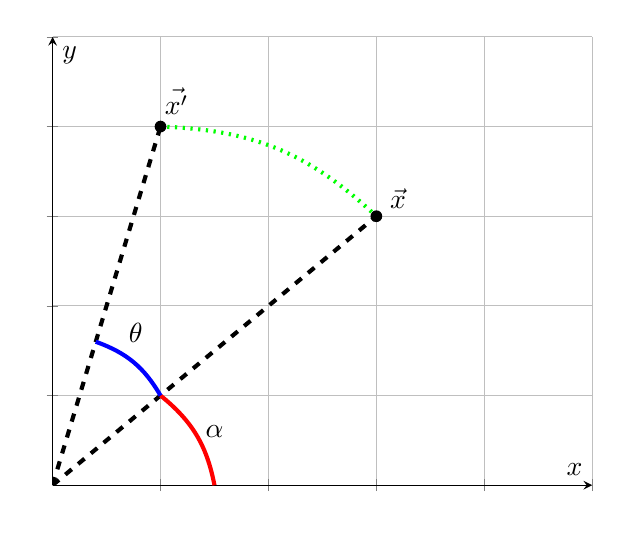
\begin{tikzpicture}
        \begin{axis}[
            grid = major,
            axis lines = center,
            xmin = 0,
            xmax = 5,
            ymin = 0,
            ymax = 5,
            xticklabels = {},
            yticklabels = {},
            xlabel = {$x$},
            ylabel = {$y$},
        ]

        \node[circle, fill, inner sep=1.5pt] (A) at (axis cs: 3, 3) {};
        \node[] at (axis cs: 3.2, 3.2) [] {$\vec{x}$};

        \node[circle, fill, inner sep=1.5pt] (B) at (axis cs: 1, 4) {};
        \node[] at (axis cs: 1.15, 4.28) [] {$\vec{x'}$};

        \addplot[line width=1.5pt, dashed, domain=0:3]{x};
        \addplot[line width=1.5pt, dashed, domain=0:1]{4*x};

        \draw[thick, dotted, green, line width=1.5pt] (A) to [bend right=20] (B);

        \draw[thick, red, line width=1.5pt] (axis cs: 1.5, 0) to [bend right=20] (axis cs: 1, 1);

        \draw[thick, blue, line width=1.5pt] (axis cs: 1, 1) to [bend right=20] (axis cs: 2/5, 8/5);

        \node[] at (axis cs: 1.5, .6) [] {$\alpha$};
        \node[] at (axis cs: .77, 1.7) [] {$\theta$};
            
        \end{axis}
    \end{tikzpicture}
\end{center}
We can represent $\vec{x}$ in polar coordinates as
\[
    x = r\cos\alpha \text { and } y = r\sin\alpha
\]
Then, 
\[
    x' = r\cos\left(\alpha + \theta\right) \text{ and } y' = r\sin\left(\alpha + \theta\right)
\]
This gives,
\begin{align*}
    x' &= r\cos\left(\alpha + \theta\right) = \overbrace{r\cos\alpha}^{x}\cos\theta - \overbrace{r\sin\alpha}^{y}\sin\theta = x\cos\theta - y\sin\theta \\
    y' &= \underbrace{r\sin\alpha}_{y}\cos\theta + \underbrace{r\cos\alpha}_{x}\sin\theta = x\sin\theta + y\sin\theta \\
    &\Rightarrow \begin{pmatrix} x' \\ y' \end{pmatrix} = 
    \begin{pmatrix}
        \cos\theta & -\sin\theta \\ 
        \sin\theta & \cos\theta
    \end{pmatrix}
    \begin{pmatrix}
        x \\ y
    \end{pmatrix}
\end{align*}

\newpage 

\begin{example}{Prove $\mathcal{T}$ is a Linear Transformation}{}
    Consider a transformation $\mathcal{T}$ such that 
    \[\mathcal{T}\left(\vec{x}\right) = 
    \begin{pmatrix}
        0 \\ x_1 + x_2 \\ x_2 + x_3 \\ x_3 + x_4
    \end{pmatrix}\]
    determine if $\mathcal{T}$ is a linear transformation.
    \begin{solution}
        Notice that $\mathcal{T}\left(\vec{x}\right) = A\vec{x}$ for 
        \[
            \underset{4 \times 4}{A} = \begin{pmatrix}
                0 & 0 & 0 & 0 \\
                1 & 1 & 0 & 0 \\
                0 & 1 & 1 & 0 \\
                0 & 0 & 1 & 1
            \end{pmatrix}
            \text{ and }
            \underset{4 \times 1}{\vec{x}} = \begin{pmatrix}
                x_1 \\ x_2 \\ x_3 \\ x_4
            \end{pmatrix}
        \]
        Because $\mathcal{T}$ can be put in the form $\mathcal{T}\left(\vec{x}\right) = A\vec{x}$, it must be a linear transformation.
    \end{solution}
\end{example}

\begin{example}{Determine if $\mathcal{T}$ is One-to-one or Onto}{}
    Consider the linear transformation $\mathcal{T}$ from the above example. Determine if $\mathcal{T}$ is one-to-one, onto, both, or neither.
    \begin{solution}
        \[
            \underset{4 \times 4}{A} = \begin{pmatrix}
                0 & 0 & 0 & 0 \\
                1 & 1 & 0 & 0 \\
                0 & 1 & 1 & 0 \\
                0 & 0 & 1 & 1
            \end{pmatrix} 
            \xrightarrow{R_1 \leftrightarrow R_4}
            \begin{pmatrix}
                1 & 1 & 0 & 0 \\
                0 & 1 & 1 & 0 \\
                0 & 0 & 1 & 1 \\
                0 & 0 & 0 & 0 
            \end{pmatrix} 
        \]
        Thus, $\text{rank}\left(A\right) \ne 4 = m = n$ so $\mathcal{T}$ is neither one-to-one nor onto.
    \end{solution}
\end{example}

\begin{example}{Find the Matrix $A$}{}
    Given that $\mathcal{T}$ is a linear transformation such that 
    \[
        \mathcal{T}\left(\vec{x}\right) = 
        A\begin{pmatrix} x_1 \\ x_2 \\ x_3 \end{pmatrix} = 
        \begin{pmatrix}
            2x_1 - 3x_2 \\
            4x_1 \\
            x_1 - x_2 + x_3
        \end{pmatrix}
    \]
    determine the value of the matrix $A$.
    \begin{solution}
        We can find $A$ as the coefficent matrix of $\mathcal{T}$:
        \[
            A = \begin{pmatrix}
               2 & -3 & 0 \\
               4 & 0 & 0 \\
               1 & -1 & 1 
            \end{pmatrix}
        \]
    \end{solution}
\end{example}

\begin{example}{Determine if $\mathcal{T}$ is One-to-one or Onto}{}
    Consider the linear transformation $\mathcal{T}\left(\vec{x}\right) = A\vec{x}$ such that $A$ is the matrix in the above example. Determine if $\mathcal{T}$ is one-to-one, onto, both, or neither.
    \begin{solution}
        We can easily figure this out by looking at the rank of $A_{\text{REF}}$. 
        \[
            A \xrightarrow[R_2 \leftrightarrow R_1]{R_2 \to \frac{1}{4}R_2}
            \begin{pmatrix}
                1 & 0 & 0 \\
                2 & -3 & 0 \\
                1 & -1 & 1
            \end{pmatrix}
            \xrightarrow[R_3 \to R_3 - R_1]{R_2 \to R_2 - 2R_1}
            \begin{pmatrix}
                1 & 0 & 0 \\
                0 & -3 & 0 \\
                0 & -1 & 1
            \end{pmatrix}
            \xrightarrow[R_2 \to -\frac{1}{3}R_3]{R_3 \to R_3 + R_2}
            \begin{pmatrix}
                1 & 0 & 0 \\
                0 & 1 & 0 \\
                0 & 0 & 1
            \end{pmatrix}
        \]
        Thus, $\text{rank}\left(A_{\text{RREF}}\right) = 3 = m = n$ so $\mathcal{T}$ is both one-to-one and onto.
    \end{solution}
\end{example}